\documentclass[main.tex]{subfiles}
\begin{document}
\chapter{Introduction} \label{sec:intro}
The understanding of elementary particles and their interactions is undoubtedly one of the most fascinating quests of the scientific endeavour. Modern particle physics has proven remarkably successful at explaining phenomena which occur at size scales orders of magnitude smaller than what our brains evolved to comprehend. The Standard Model (SM), which is a collection of Quantum Field Theories (QFTs) that describe the subatomic world, allows us to rigorously test our ideas about how the Universe functions at the most bare, fundamental level. It relies on a constant interplay between theoretical predictions and their experimental verification (or negation). From the perspective of a theoretical physicist, it is crucial to be able to derive increasingly precise predictions for physically observable quantities that can be measured in particle colliders such as the Large Hadron Collider (LHC) at CERN. This theoretical precision should match what can be achieved experimentally. The growing amount of data from Run 3 at the LHC makes this a challenge for the theoretical community, pushing us to constantly improve our computational tools in order to refine our predictions. 

The subject of this thesis is precisely the story of trying to overcome the current limitations in an effort to exploit the predictive power of QFT to an even greater extent. It is a famous fact of physics that QFT computations cannot be performed exactly, apart from the most trivial cases. Instead, one follows an approximate description through the so-called perturbation theory. In this approach, the leading-order (LO) terms in the computation are low in number and complexity. They represent a crude, almost `back-of-the-envelope' estimation of the full answer. The next-to-leading-order (NLO) terms increase in number and are harder to calculate. Nonetheless, they provide a refinement of the LO result and are absolutely necessary for precision phenomenology. Roughly speaking, the cutting edge of QFT computations is currently at the next-to-next-to-leading-order (NNLO) for $2 \rightarrow 3$ processes and at N$^3$LO for $2 \rightarrow 2$ processes. They can involve millions of individual terms, each of which can be incredibly hard to evaluate. 

In this thesis, we will focus on the description of one of the key ingredients needed for QFT computations, i.e. the scattering amplitudes. We hope to provide the reader with detailed understanding of why they are important in the first place, how they are calculated and the difficulties that we have to overcome in practice. Naturally, we cannot jump into full detail straightaway. We hope that this thesis will be approachable to someone who already possesses basic knowledge of QFT, but we certainly do not assume previous experience in this topic at research level. For this reason, we dedicate the rest of Chapter~\ref{sec:intro} to reviewing the rudimentary information needed further on. This content should be familiar from a thorough introductory course to QFT. Next, in Chapter~\ref{sec:tools} we introduce more advanced and specialised techniques that are used to compute scattering amplitudes. We hope that despite the breadth of the concepts covered and often heavy mathematical detail, this chapter will not be too hard to follow. Our reward will come in the following chapters, where we will use the techniques described thus far to compute scattering amplitudes necessary for the NNLO description of three selected processes. We will focus on amplitudes which are relevant to processes that have been deemed of high priority by the particle physics community. The biannual Les Houches report provides a wishlist of processes whose improved theoretical description would greatly contribute to our understanding of fundamental particles~\cite{Huss:2022ful}. Amongst others, two-loop QCD amplitudes relevant to Higgs boson production in association with a bottom-quark pair, $\ppbbh$, as well as to $W^\pm$ boson production with a photon and a jet, $\ppWgj$, are highly desired. They are described in Chapters~\ref{sec:Hbb} and \ref{sec:Wyj} and represent some of the first results for five-point processes with an external massive leg at this loop order. In Chapter~\ref{sec:QEDpaper}, we switch our focus to the QED process $0 \to l \bar{l} \gamma \gamma^\ast$, which is required to achieve the precision goal of the MUonE experiment. For this purpose, we will construct a basis of special functions for integrals needed to describe any four-point process with one external massive leg at the two-loop order. Finally, in Chapter~\ref{sec:conclusions}, we draw our conclusions and discuss directions for future work.

\section{QFT background} \label{sec:QFTintro}
The rest of this introduction is meant to provide the reader with a bridge between elementary knowledge of QFT and state-of-the-art techniques that are used to extract predictions from it. We start by providing a brief summary of the relevant information about QFTs, and in particular QCD. Next, in Section~\ref{sec:particlescattering} we describe how to connect this theory to physical observables that can be measured experimentally. This introduces the notion of a scattering amplitude in Section~\ref{sec:fromcrosssectoamps}, which will be the main focus of this thesis. Finally, in Section~\ref{sec:divergences} we discuss the famous problem of divergences present in QFT computations and show how in the process of trying to keep them under control, we discover a surprising feature of QCD interactions. At the end, we will be ready to tackle the more advanced topics presented in Chapter~\ref{sec:tools}.

One of the central equations of QFT, which describes all spin\=/1/2 particles, is the Dirac equation:
\begin{equation} \label{eq:Dirac}
    (\ii \slashed{\partial}-m)\psi(x) = 0\,.
\end{equation}
Its solutions are given by the four-component Dirac spinors $\psi(x)$, which transform in the irreducible $\left(\frac{1}{2}, 0\right) \otimes \left(0, \frac{1}{2}\right)$ representation\footnote{Not to be confused with the usual four-vectors $x^\mu$, which transform in the $\left(\frac{1}{2}, \frac{1}{2}\right)$ representation.}. There are four plane-wave solutions, which admit both positive and negative frequencies:
\begin{equation}
    \psi(x) = u^s(p)\ex{-\i p\cdot x} \qquad \text{and} \qquad \psi(x) = v^s(p)\ex{+\i p\cdot x}\,,
\end{equation}
where $s \in \{1, 2\}$. The momentum space spinors $u(p)$ and $v(p)$ are interpreted as describing particles and antiparticles with \textit{positive} energies. They satisfy the momentum space Dirac equations: 
\begin{align}
    (\slashed{p} - m)u(p) &= 0\,, \nonumber \\
    (\slashed{p} + m)v(p) &= 0\,,
\end{align}
as well as the following completeness relations, which are useful when performing spin sums in QFT computations:
\begin{align} \label{eq:completeness:fermions}
    \sum_{s \in \{1,\, 2\}} u^s(p)\bar{u}^s(p) &= \slashed{p} + m\, \nonumber, \\
    \sum_{s \in \{1,\, 2\}} v^s(p)\bar{v}^s(p) &= \slashed{p} - m\,.
\end{align}
Moreover, it is convenient to split the spinors into two separate components:
\begin{equation}
    \psi(x) = 
    \begin{pmatrix}
        \psi_L(x) \\
        \psi_R(x)
    \end{pmatrix}\,,
\end{equation}
where the left- and right-handed Weyl spinors $\psi_L(x)$ and $\psi_R(x)$ transform in the $\left(\frac{1}{2}, 0 \right)$ and $\left(\frac{1}{2}, 0 \right)$ representations, respectively. It is important to note that Eq.~\ref{eq:Dirac} mixes these two components, which can be appreciated by writing it explicitly in matrix notation. In the so-called Weyl (or chiral) basis, the Dirac matrices are:
\begin{equation}
    \gamma^\mu = 
    \begin{pmatrix}
        0 & \sigma^\mu \\
        \bar{\sigma}^\mu & 0
    \end{pmatrix}\,,
\end{equation}
with $\sigma^\mu \equiv (\mathds{1}, \sigma^i)$ and $\bar{\sigma}^\mu \equiv (\mathds{1}, -\sigma^i)$, and $\sigma^i$ for $i=1,2,3$ are the Pauli matrices. Thus, the Dirac equation is:
\begin{equation}
    \begin{pmatrix}
        -m & \ii \sigma^\mu \partial_\mu \\
        \ii \bar{\sigma}^\mu \partial_\mu & -m \\
    \end{pmatrix}
    \begin{pmatrix}
        \psi_L(x) \\
        \psi_R(x)
    \end{pmatrix} = 0 \,,
\end{equation}
where each entry is in itself understood to be a $(2 \times 2)$ matrix. Crucially, we can see that in the absence of mass, the two components fully decouple and can be treated separately. It is also useful to define an additional $\gamma^5$ matrix: 
\begin{equation}
    \gamma^5 \equiv \i \gamma^0 \gamma^1 \gamma^2 \gamma^3\,,
\end{equation}
which in the Weyl representation is just:
\begin{equation}
    \gamma^5 = 
    \begin{pmatrix}
        -\mathds{1} & 0 \\
        0 & \mathds{1}
    \end{pmatrix}\,.
\end{equation}
The fifth $\gamma$-matrix plays a surprisingly important role in QFT. First, the Weyl spinors can be extracted from the Dirac spinors by applying appropriate projectors:
\begin{equation}
    P_L = \frac{\mathds{1}-\gamma^5}{2} = 
    \begin{pmatrix}
        \mathds{1} & 0 \\
        0 & 0
    \end{pmatrix}\,,
    \qquad
    P_R = \frac{\mathds{1}+\gamma^5}{2} = 
    \begin{pmatrix}
        0 & 0 \\
        0 & \mathds{1}
    \end{pmatrix}\,,
\end{equation}
according to $\psi_L(x) = P_L\psi(x)$ and $\psi_R(x) = P_R\psi(x)$. This allows us to associate $\psi_L$ and $\psi_R$ with the helicity of a particle, which is the projection of its spin onto the direction of motion. The corresponding helicity values for left- and right-handed particles are $-1$ and $+1$, respectively\footnote{Strictly speaking, the left- and right-handed Weyl spinors are eigenstates of the chirality operator $\gamma^5$. However, for $m=0$, helicity and chirality eigenstates coincide.}. Weyl spinors will play a key role in the discussion of the spinor-helicity formalism in Section~\ref{sec:spinhelform}. Moreover, the $P_L$ projector appears in the $V-A$ coupling of the charged $W^\pm$ bosons to quarks and leptons, reflecting the fact that they interact only with left-handed fermions. Finally, as we will see in Sections~\ref{sec:Hbb} and ~\ref{sec:Wyj}, $\gamma^5$ allows us to introduce a pseudo-scalar invariant which is needed to capture the parity information of the kinematic phase-space. 

Apart from fermions, we also need to know how to deal with bosons. In particular, spin\=/1 bosons are described by vector fields $A^\mu$, which transform in the $(\frac{1}{2}, \frac{1}{2})$ representation of the Lorentz group. For the massive gauge bosons, that is $W^\pm$ and $Z^0$, imposing their equations of motion leads to three distinct solutions labelled $\varepsilon_\mu^s(p)$ and referred to as polarisation vectors.
Similarly to the completeness relations for spin\=/1/2 fermions, Eq.~\ref{eq:completeness:fermions}, the polarisation vectors of the massive gauge bosons satisfy the following property:
\begin{equation}
    \sum_{s \in \{0,1,2\}} \eps_\mu^s(p) (\eps_\nu^s(p))^{\ast} = -g_{\mu\nu} + \frac{p_\mu p_\nu}{M^2} \,,
\end{equation}
%Eq. 21.26 in Peskin or 85.16 in Srednicki (but remember he uses -+++ metric)
On the other hand, massless gauge bosons, i.e. photons and gluons, have only two polarisations, which can be interpreted as helicity eigenstates. Their completeness relation reads:
\begin{equation} \label{eq:completeness:bosons}
    \sum_{s \in \{-,+\}} \eps_\mu^s(p, q) (\eps_\nu^s(p, q))^{\ast} = -g_{\mu\nu} + \frac{p_\mu q_\nu + p_\nu q_\mu}{p \cdot q} \,,
\end{equation}
where $q^\mu \neq p^\nu$ is an arbitrary reference vector which is introduced to help decompose the four-component vectors $\varepsilon^\mu$ into two-component objects, similarly to the decomposition of the Dirac spinor into Weyl spinors. The end result of any computation is independent of $q^\mu$, which reflects gauge invariance (we will elaborate on this fact in Section~\ref{sec:spinhelform}). 

Finally, the Standard Model famously includes a scalar particle --- the Higgs boson. This boson is responsible for electroweak symmetry breaking and, as a direct consequence, giving mass to the electroweak gauge bosons $W^\pm$ and $Z^0$. 
\section{Quantum Chromodynamics} \label{sec:QCD}
In this thesis, we will concern ourselves with the study of interactions involving mainly quarks and gluons. As such, a brief refresher of the relevant information is in order. SM particles carrying colour charge interact via the strong force, which is mathematically described by QCD. Its Lagrangian can be schematically represented as a sum of three parts:
\begin{equation}
    \mathcal{L}_{\text{QCD}} = \mathcal{L}_{\text{classical}} + \mathcal{L}_{R_\xi} + \mathcal{L}_{\text{ghosts}}\,.
\end{equation}
We begin by discussing the classical part. It is given by:
\begin{equation} \label{eq:QCDLagrangian}
    \mathcal{L}_{\text{classical}} = -\frac{1}{4} G^a_{\mu\nu} G^{a\,\mu\nu} + \sum_q^{n_f} \overline{\psi}_{q}^{\,i} \left(\ii \slashed{D}_{ij} - m_q \delta_{ij} \right) \psi_q^j\,,
\end{equation}
where:
\begin{equation}
     G^a_{\mu\nu} = \partial_\mu A^a_\nu + \partial_\nu A^a_\mu + g_s f^{abc} A^b_\mu A^c_\nu
\end{equation}
is the gluon field strength, while:
\begin{equation}
    (D_\mu)_{ij} = \delta_{ij} \partial_\mu - \ii g_s (T^a)_{ij} A^a_\mu
\end{equation}
is the covariant derivative introduced to ensure gauge invariance under SU($N_c$) transformations\footnote{We will keep the degree $N_c$ of the group SU($N_c$) generic in the discussion below, but of course we are interested in the QCD case of $N_c=3$.}.

The QCD Lagrangian contains three types of fields. Quarks and antiquarks, corresponding to $\psi_q^i$ and $\overline{\psi}_q^{\,i}$, respectively, transform in the fundamental and antifundamental representations of SU($N_c$). In QCD, they have $n_f = 6$ flavours. The indices $i \in \{1,\ldots,N_c\}$ denote the colour charge of the (anti)quarks. It is common to drop the colour index and write $\psi_q$, which is understood as $\psi_q \equiv \left(\psi_q^r, \psi_q^b, \psi_q^g \right)^T$. The fundamental fields are acted on by the $N_c^2-1$ fundamental generators of SU($N_c$) with dimensions $(N_c \times N_c)$. For SU(3), they are given by:
\begin{equation}
    (T^a)_{ij} = \frac{1}{2} (\tau^a)_{ij}\,,
\end{equation}
where $(\tau^a)_{ij}$ are the eight $(3 \times 3)$ Gell-Mann matrices. Similarly, the antifundamental fields are acted on by the generators in the antifundamental representation, $\overline{T}^{\,a} = -\left(T^a\right)^\ast$. The fundamental generators are normalised according to:
\begin{equation}
    \tr (T^aT^b) = T_F \delta^{ab},
\end{equation}
with $T_F = \frac{1}{2}$ in QCD. Finally, let us list one more extremely useful relation they satisfy:
\begin{equation} \label{eq:fierzcolour}
    (T^a)_{ij} (T^a)_{kl} = T_F \left( \delta_{il} \delta_{jk} - \frac{1}{N_c} \delta_{ij} \delta_{kl} \right)\,,
\end{equation}
which is known as the Fierz identity.

The third type of field, the gluon field, is represented by $A^a_\mu$. It transforms in the adjoint representation, i.e. under the action of $N_c^2-1$ adjoint generators with dimensions $(N_c^2-1 \times  N_c^2-1)$:
\begin{equation}
\left(T_\text{adj}^a\right)^{bc} = -\ii f^{abc}\,,
\end{equation}
where $a,b,c \in \{1, \ldots, N_c^2-1\}$ are the colour indices and the totally antisymmetric objects $f^{abc}$ are known as the structure constants. Typically, the adjoint generators are normalised such that $\tr (T_\text{adj}^aT_\text{adj}^b) = N_c \delta^{ab}$. 

SU($N_c$) generators (in any representation) satisfy the following defining relation of the Lie algebra:
\begin{equation} \label{eq:liealgebra}
    \left[T^a, T^b\right] = \ii f^{abc} T^c\,.
\end{equation}
Note that for Abelian groups, the structure constants vanish. For the non-Abelian SU(3) group of QCD, they are non-vanishing and it is useful to invert the above relation in terms of the fundamental generators:
\begin{equation} \label{eq:fabc}
    f^{abc} = -\frac{\ii}{T_F} \tr \left(\left[T^a, T^b \right] T^c \right)\,.
\end{equation}
Thus, the structure constants, which are associated with 3- and 4-gluon vertices in Feynman diagrams, can be written in terms of traces of fundamental generators. This fact, along with the Fierz identity, becomes very useful when computing scattering amplitudes in QCD, as we will see in Section~\ref{sec:colourdec}.

In the process of deriving the QCD gluon propagator, the notion of gauge invariance leads to two important qualitative features. First of all, just as in the case of the photon propagator in QED, instead of explicitly fixing the gauge, we find it convenient to introduce an auxiliary (i.e. non-propagating) field $\xi$. We write:
\begin{equation} \label{eq:gaugefixing}
    \mathcal{L}_{R_\xi} = -\frac{1}{2 \xi} \left(\partial^\mu A^a_\mu \right)^2\,,
\end{equation}
which yields the gluon propagator:
\begin{equation}
    \Pi^{\mu\nu}(p) = \frac{-\ii \, \delta^{ab}}{p^2+ \ii \varepsilon} \left(g^{\mu\nu} - (1-\xi) \frac{p^\mu p^\nu}{p^2+\ii \varepsilon} \right)\,.
\end{equation}
As an example, with term Eq.\ref{eq:gaugefixing} included in the full QCD Lagrangian, for small $\xi$ we must have that $\partial^\mu A^a_\mu \rightarrow 0$ in order to prevent the exponential of $\mathcal{L}$ from blowing up, such that we can still minimise the action. Thus, the choice $\xi = 0$ is equivalent to the Lorenz gauge and spares us from having to impose the Lorenz condition throughout the entire computation. Other choices are possible, of course. In fact, the most common prescription is to set $\xi = 1$, which is known as the Feynman-'t Hooft gauge. It is also possible to keep $\xi$ generic --- gauge invariance ensures that the results of computations of physical quantities will at the end be free of $\xi$.

The second feature, which appears only in non-Abelian gauge theories, is that gauge fixing the Lagrangian implies that not only the physical transverse modes of $A^a_\mu$ can propagate. To cancel the unphysical degrees of freedom propagating through gluon loops in Feynman diagrams, it is necessary to include in the Lagrangian Grassmann-valued fields $c$ and $\bar{c}$ representing Faddeev-Popov ghosts and antighosts:
\begin{equation} \label{eq:ghosts}
    \mathcal{L}_\text{ghosts} = (\partial^\mu \bar{c}^{\,a})(\delta^{ac} \partial_\mu + g_s f^{abc} A^b_\mu ) c^c\,.
\end{equation}
These particles are not physical states. In fact, it is possible to work in non-covariant gauges, such as the axial gauge or the lightcone gauge, where ghosts decouple from physical particles and can be neglected. However, the cost of doing so is a more complicated expression for the gluon propagator, which may lead to tougher computations. Thus, we usually accept ghosts as a peculiarity of working with non-Abelian gauge theories and include them in our computations. They couple only to gluons (and not to quarks) and receive their own Feynman rules for the propagator and the vertex.

\section{Particle scattering} \label{sec:particlescattering}
Having introduced the QFTs that describe the most fundamental particles our nature has to offer, one might rightfully wonder about the rewards for our intellectual effort (beyond personal satisfaction). After all, amongst our non-physicist friends, it is common to think that the word `theoretical' in `theoretical physics' is synonymous with `hypothetical'. Not much could be further from the truth and we dedicate this section to illustrating the immense predictive power of QFTs.

Consider a typical particle physics experiment. Two beams of particles, travelling in opposite directions, interact briefly and produce a host of new states that fly away in various directions until they are registered by some kind of a detector. Naturally, the number of such scattering events is proportional to the number of particles in the two beams, $N_a$ and $N_b$, as well as to the area common to the beams, $A$. The ratio of these quantities is known as the scattering cross section:
\begin{equation} \label{eq:crossection}
    \sigma \equiv \frac{\text{number of scattering events}}{N_a N_b A}\,.
\end{equation}
Typically, apart from just counting the total number of events, we want to differentiate between the type of outgoing particles, their momentum, angle of collision, etc. However, if we specify an exact value for a continuous variable such as the momentum, the numerator of Eq.~\ref{eq:crossection} becomes infinitesimal. To avoid this issue, we usually work with a \textit{differential} cross section, e.g. $\dd\sigma/(\dd p_1 \ldots \dd p_n)$, such that its integral over some small range of $p_i$ gives the \textit{total} cross section in that region of momentum space. While cross sections can be measured in particle colliders, it is the task of QFT to make predictions for them.

In the case of hadron collisions, there is one additional complication which needs to be taken into account. The fundamental objects of QCD are quarks and gluons, however they cannot be observed individually due to colour confinement --- only their colourless combinations can be detected in a collider. The LHC, being a proton-proton collider, requires a more complicated model of the interactions than just the scattering of point particles. As we will soon see, QCD exhibits a behaviour known as asymptotic freedom. That is, the coupling $\alpha_s$ decreases with energy (i.e. at small distances) and its value determines whether we are allowed to use perturbation theory or not. Roughly speaking, above the scale $\Lambda_\text{QCD} \sim 200 \text{ MeV}$, $\alpha_s$ becomes small enough so that the perturbative expansion is justified. The individual `partons' (i.e. quarks, antiquarks and gluons) act like free particles and undergo `hard' scattering\cite{PhysRevLett.23.1415}. On the other hand, physics at energies below $\Lambda_\text{QCD}$ is necessarily non-perturbative due to large $\alpha_s$ values. Its effects are captured by the Parton Distribution Functions (PDFs) $f_i(x, \mu_F)$, which give the probability of finding in a hadron a given parton $i$ with momentum fraction $x$ of this hadron. Here, $\mu_F$ is a factorisation scale which separates the high and low-energy physics. In fact, the PDFs run with $\mu_F$, similarly to the running of the QCD coupling $\alpha_s$, and their evolution is given by the DGLAP equations\footnote{The origin of $\mu_F$ will be discussed in more detail in Section~\ref{sec:IRdivergencesandKLN}.}. Overall, the factorisation of soft and hard physics allows us to write the cross section for the scattering of two hadrons $h_1, h_2$ to the final state $X$ as~\cite{Collins:1989gx}:
\begin{equation} \label{eq:factorisation}
    \dd \sigma_{h_1 h_2 \to X} = \sum_{i,j} \int_0^1 \dd x_1 \dd x_2 \, f_i(x_1, \mu_F) f_j(x_2, \mu_F) \, \dd \hat{\sigma}_{ij \to X}\left(\mu_F, \mu_R, Q^2\right) + \order{\frac{\Lambda_\text{QCD}^2}{Q^2}}\,,
\end{equation}
where $i, j$ are the partons of hadrons $h_1$ and $h_2$, respectively, and $\hat{\sigma}_{ij \to X}$ is the \textit{partonic} cross section for the scattering of $i,j$ into the final state. The higher-order terms can be neglected as long as the scale $Q$ at which we are probing the hard scattering is significantly greater than $\Lambda_{\text{QCD}}$. Since the PDFs describe effects at large $\alpha_s$, they cannot be calculated using perturbative QCD. Instead, they are extracted from experimental data (see e.g. Refs.~\cite{H1:2015ubc, Alekhin:2017kpj, Hou:2019efy, NNPDF:2021uiq, Buckley:2014ana}). On a positive note, they are universal, i.e. process independent, so once they have been determined from some experiment, they can be re-used in the description of any other hadron interaction.

Contrary to the PDFs, the partonic cross sections are computed using perturbative QCD. Before turning our full attention to these objects, let us briefly remark that even after the scattering has taken place, a lot of interesting physics is still ongoing (see Fig.~\ref{fig:collision}). The final state partons can radiate a cascade of other partons in a phenomenon referred to as parton showers. Furthermore, these coloured partons cannot be detected in a collider --- as the energy scale falls below $\Lambda_\text{QCD}$, they combine together to form colourless hadrons. Finally, unstable hadrons may decay into further products. What is actually detected in a collider is then a collimated spray of hadrons and other particles referred to as a jet. Using the so-called jet algorithms and definitions, one then tries to reverse engineer the collision of individual partons. We refer the reader to Refs.~\cite{Plehn:2009nd, Hoche:2014rga} for a closer look at these topics.
\begin{figure}
    \begin{center}
        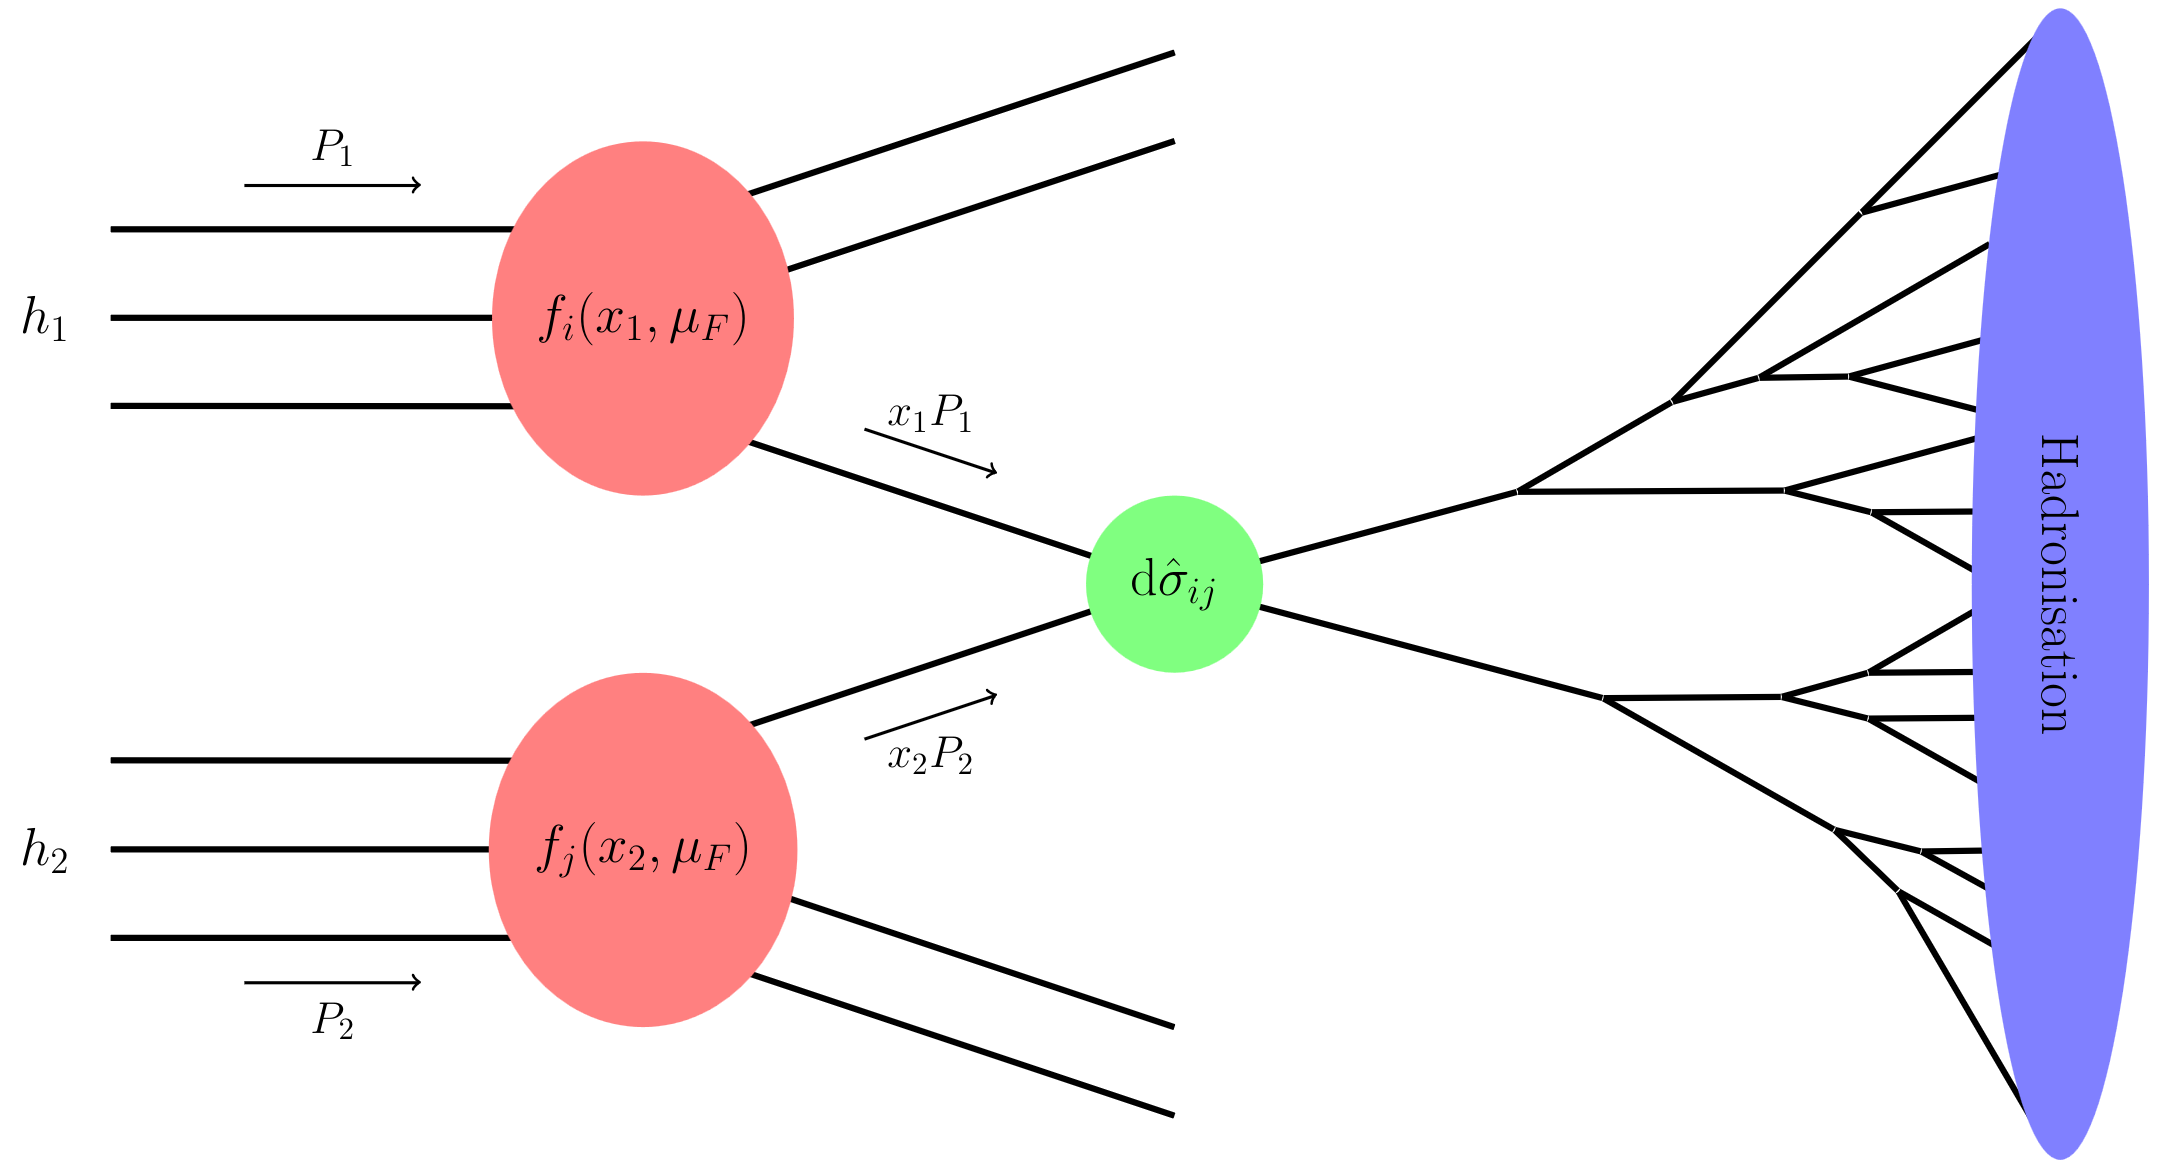
\includegraphics[width=0.8\textwidth]{img/collision.png}
        \caption{
            A schematic representation of a collision between two hadrons, $h_1$ and $h_2$, with total momenta $P_1, P_2$. A parton $i$ carrying momentum $x_1 P_1$ undergoes hard scattering with a parton $j$ carrying momentum $x_2 P_2$. Their factorisation from hadrons is described by the PDFs $f_i(x_1, \mu_F)$ and $f_j(x_2, \mu_F)$, while their interaction is described by the partonic cross section $\dd\hat\sigma_{ij}$. The splitting lines represent subsequent parton showers, which then undergo hadronisation as the energy scale falls below $\Lambda_\text{QCD}$. Further decays and jets are not shown. Image courtesy of Ryan Moodie~\cite{Moodie:2022dxs}.
        }
        \label{fig:collision}
    \end{center}
\end{figure}

\section{From cross sections to scattering amplitudes} \label{sec:fromcrosssectoamps}
Having decoupled the high and low energy physics within a hadron, let us now address the computation of the hard scattering between partons. The partonic cross section $\hat{\sigma}_{i\rightarrow f}$ is simply related to the probability of starting with some initial state $i$ and ending up with the final state $f$, that is: $\mathcal{P} = |\braket{f|i}|^2$. These interacting states are not the free wave packets with well-defined momenta that we know how to handle using the QFT machinery. However, they do become free in the limit as $t\rightarrow -\infty$, i.e. before the interaction, as well as $t \rightarrow \infty$, i.e. after the interaction. The idea is then to view the scattering in the following way: an asymptotically free state $\ket{i}_{t=-\infty}$ evolves to a real-world state $\ket{i}$, undergoes scattering (of negligible duration) into the state $\ket{f}$ which finally evolves into the free state $\ket{f}_{t=\infty}$. The evolution of real states from and to the asymptotic states is captured by the $S$-matrix, which is calculated from the Hamiltonian in the interaction representation. Specifying to the scattering of two partons into $n-2$ particles, we write the so-called $S$-matrix elements in terms of the free multi-particle states:
\begin{equation} \label{eq:Smatrixelements}
    \braket{p_3, \ldots, p_n|S|p_1,p_2}\,.
\end{equation}
Furthermore, it is customary to split the $S$-matrix according to:
\begin{equation} \label{eq:StoiT}
    S = \mathds{1} + \i T\,.
\end{equation}
In any scattering experiment, there is a large chance of the particles simply missing each other and nothing happening, which is expressed by the identity matrix. The interesting physics of interactions is captured by the transition matrix $T$:
\begin{equation} \label{eq:Tmatamplitudes}
    \braket{p_3, \ldots, p_n|\i T|p_1,p_2} = (2\pi)^4 \delta^{(4)}\left(p_1+p_2 - \sum_{f=3}^n p_f\right)\, \i \mathcal{A} (p_1,p_2 \rightarrow p_3, \ldots, p_n) \,,
\end{equation}
where we included the overall $\delta$-function to impose 4-momentum conservation. Here, $\mathcal{A} (p_1,p_2 \rightarrow p_3, \ldots, p_n)$ is the $n$-particle \textbf{scattering amplitude}. Finally, to relate the amplitudes to the partonic cross section, we insert Eq.~\ref{eq:Tmatamplitudes} into Eq.~\ref{eq:Smatrixelements} and integrate over a small region $\dd^3p_3 \ldots \dd^3 p_n$. This integration encodes the probability that the $n-2$ final particles will belong to that region of the momentum phase-space. Overall, the recipe reads:
\begin{equation} \label{eq:crosssecampl}
    \dd \hat{\sigma} = \frac{1}{2E_1 2E_2 |v_1-v_2|} \left(\prod_f \frac{\dd^3 p_f}{(2\pi)^3} \frac{1}{2E_f} \right) (2\pi)^4 \delta^{(4)}\left(p_1+p_2 - \sum_f p_f\right)|\mathcal{A}(p_1,p_2 \rightarrow p_f)|^2\,.
\end{equation}
The first term in this formula is a flux factor related to the relative velocity of the two incoming beams in the laboratory reference frame, $|v_1-v_2|$. Next, the overall $\delta$-function imposes Lorentz invariance on the phase-space integration over $\prod_f \dd^3 p_f$. In practice, the phase-space integration is carried out using Monte Carlo event generators~\cite{Reuschle:2014fya, Campbell:2022qmc}. Finally, the formula is completed by the square of the scattering amplitude.

Scattering amplitudes therefore represent a vital bridge between theory an experiment. On one hand, due to Eq.~\ref{eq:crosssecampl}, they allow us to derive predictions for physical observables that can be measured in a collider. On the other hand, due to their connection with the $S$-matrix through Eq.~\ref{eq:Tmatamplitudes}, they are sensitive to our understanding of the underlying theory of interactions. As such, computing amplitudes serves as a key tool to challenge and improve our models of elementary particles. Unfortunately, in all but the simplest cases, the $S$-matrix elements cannot be calculated exactly. Instead, we resort to an expansion in powers of the coupling constant:
\begin{equation} \label{eq:ampexpansion}
    \ampl{n}{} = \alpha^t \left(\ampl{n}{(0)} + \alpha^1 \ampl{n}{(1)} + \alpha^2 \ampl{n}{(2)} + \ldots \right) \,.
\end{equation}
In this formula, each term is calculated from linear combinations of expressions corresponding to Feynman diagrams. The expansion starts at the power $t$ of the LO term $\ampl{}{(0)}$. This term usually --- but not always --- corresponds to tree-level diagrams, i.e. diagrams with no closed loops. Higher-order terms $\ampl{}{(L)}$ gain additional powers of $\alpha$ due to $L$-loop diagrams. Therefore, at high energies where the coupling constant becomes small, we can approximate the full scattering amplitude by truncating the expansion in Eq.~\ref{eq:ampexpansion} at a desired order.

Let us stress that the computation of each element described so far, i.e. the cross sections, PDFs, the phase-space integration, amplitudes, parton showers, hadronisation and jets, is a tremendous effort undertaken by a multitude of particle physicists around the world. This thesis is a small building block of the entire enterprise and aims to shed light on just one of these aspects --- the calculation of scattering amplitudes.

\section{Divergences and dimensional regularisation} \label{sec:divergences}
Let us now devote our attention to the study of Feynman integrals and diagrams, a fundamental tool used to compute scattering amplitudes. For a tree-level diagram, all momenta are uniquely fixed by momentum conservation at the vertices and no integration is necessary. However, the presence of loops introduces an unconstrained `loop momentum' which needs to be integrated over (see Fig.~\ref{fig:genericint}). We will denote them as $k_l$, where $1\le l\le L$. It is a famous fact of QFT that many Feynman integrals often contain divergences. They come in two types: 
\begin{itemize}
    \item \textbf{Ultraviolet divergences} --- these appear when $k \rightarrow \infty$,
\item \textbf{Infrared divergences} --- these arise in processes with massless particles and are further subdivided into:
\begin{itemize}
    \item \textbf{Soft divergences} --- when $k \rightarrow 0$,
    \item \textbf{Collinear divergences} --- when the loop momentum $k$ becomes collinear to a massless external momentum.
\end{itemize}
\end{itemize}
\begin{figure}[t]
    \centering
    \hspace{-2cm}
	\begin{tikzpicture}[scale=0.5]
        \begin{feynman}
		\filldraw[gray!50,draw=black] (0,0) ellipse (4 and 2);
		\draw[fill=white,draw=black,] (-2.5,0) ellipse (0.7cm and 1cm) node {\small $k_1$};
		\draw[fill=white,draw=black,] (-.9,0) ellipse (0.7cm and 1cm) node {\small $k_2$};
		\draw[fill=white,draw=black,] (+2.5,0) ellipse (0.7cm and 1cm) node {\small $k_L$};
        \node (ldots) at (0.8, 0) {$\ldots$};

        \node (kL) at (2.5, 0);
        \ddd{kL.center}{2.5cm}{d1}{d2}{d3}{0}{20};
		
        \draw[thick] (3, 1.32) -- (5,3) node [anchor=south west] {$p_3$};
		\draw[thick] (3, -1.32) -- (5,-3) node [anchor=north west] {$p_n$};
		\draw[thick] (-3, 1.32) -- (-5,3) node [anchor=south east] {$p_2$};
		\draw[thick] (-3, -1.32) -- (-5,-3) node [anchor=north east] {$p_1$};

        \node (text) [text width=5cm] at (12, 0.5) {\begin{equation*}
            \longleftrightarrow \qquad \prod_{l=1}^L \left( \mu_R^{2\eps} \int \frac{\dd^d k_l}{\ii \, \pi^{d/2}}\right) \frac{N}{\prod_i D_i(k,p,m)}
        \end{equation*}};
        \end{feynman}
	\end{tikzpicture}
    \caption{An $L$-loop Feynman diagram corresponds to an $L$-fold Feynman integral. We continue the integrals from $4$ to $d$ dimensions (see Section~\ref{sec:dimreg} for explanation). The numerator $N$ is determined by the Feynman rules of the underlying theory and contains objects such as momenta, spinors and polarisation vectors. The corresponding denominators have the form $D_i = (k_i+q_i)^2-m_i^2 + \ii \varepsilon$, where $q_i$ are linear combinations of external (and potentially internal) momenta and we have explicitly included the pole prescription.}
    \label{fig:genericint}
\end{figure}
\subsection{UV divergence and renormalisation}
The two types of divergences are handled in separate ways. Firstly, UV divergences are dealt with using renormalisation. In short, we start by realising that the masses, fields and couplings in the original Lagrangian of Eq.~\ref{eq:QCDLagrangian} are not `physical', in the sense that we have been using them to define the perturbative expansion, but they do not correspond to the physical parameters that can be measured in a collider. From this perspective, the fact that our attempts at deriving predictions from QFT result in an abundance of infinities does not shatter our dreams of having a sensible theory of real-world interactions. One simply needs to move these infinities away from the integrals and into the definitions of the naive, `bare' couplings. It is conventional to introduce into the Lagrangian so-called counterterms (with their own Feynman rules and diagrams) designed precisely to cancel out divergences up to a given order in perturbation theory. The inclusion of counterterms (which are themselves divergent) is equivalent to shifting the couplings from their bare values to the physical ones. This means that the predictions obtained using the physical parameters will now be UV-finite. To obtain the values of the physical parameters themselves, we need to relate them to some quantity that can be measured in an experiment. This measurement can be performed at an arbitrary energy $\mu_R$, which is known as the renormalisation scale. Then, the relationship between the bare and physical couplings allows us to write down the renormalised expression for the scattering amplitude. Even though the renormalised amplitudes are a function of the physical couplings as measured at some $\mu_R$, the choice of this renormalisation scale is arbitrary and the predictions obtained from the renormalised amplitudes are independent of it.

The renormalisation of QCD has an immediate and astounding consequence. The physical strong coupling constant is not, in fact, a constant, but rather depends on a scale: $\alpha_s = \alpha_s(\mu)$. 
%In other words, the strength of the interaction depends on the energy at which we are probing the system.
It is then natural to wonder how the coupling evolves, or `runs', with this scale. The answer to this question is given by the famous $\beta$-function, which in QCD takes the form~\cite{PhysRevD.2.1541, Symanzik:1970rt}:
\begin{equation} \label{eq:QCDbetafunction}
    \beta(\alpha_s) \equiv \frac{\dd \alpha_s}{\dd \log \mu^2} = - \sum_{i=0}^\infty \beta_i \left (\frac{\alpha_s}{4\pi} \right)^{i+2}\,.
\end{equation}
It is currently known up to five loops~\cite{Baikov:2016tgj}. Crucially, the first coefficient is:
\begin{equation}
    \beta_0 = \frac{11}{3} C_A - \frac{4}{3} T_F n_f\,,
\end{equation}
where $n_f$ is the number of light quarks, i.e. quarks with masses below the scale at which we're probing the system. With $C_A = N_c = 3$ and $T_F = 1/2$, it is clear that $\beta_0>0$ as long as $n_f\le 16$, which is of course the case in our world. Then, the overall minus sign in Eq.~\ref{eq:QCDbetafunction} means that, perhaps counterintuitively, $\alpha_s$ \textit{decreases} as we move towards higher energies. This phenomenon is known as asymptotic freedom and motivates the factorisation of amplitudes in Eq.~\ref{eq:factorisation}. Solving the renormalisation group equation Eq.~\ref{eq:QCDbetafunction} at the lowest order gives:
\begin{equation}
    \alpha_s(\mu) = \frac{2\pi}{\beta_0 \log \left(\frac{\mu}{\Lambda_\text{QCD}}\right)}\,,
\end{equation}
where $\Lambda_\text{QCD}$ arises as an integration constant and is the same scale we used in Section~\ref{sec:particlescattering} to separate the perturbative physics of high energies from the non-perturbative PDFs of low energies. 

Finally, we mention that not all theories are renormalisable, i.e. to remove all their UV divergences, we would need to add an infinite number of counterterms. Fortunately for us, QCD is indeed renormalisable (as a matter of fact, the entire Standard Model is renormalisable). As such, we can go ahead with our computation of QCD scattering amplitudes and be sure that at the end of the day, we will be able to avoid infinite predictions. For further details of renormalisation and related topics, we refer the reader to any of the standard QFT textbooks.
\subsection{IR divergences and the KLN theorem} \label{sec:IRdivergencesandKLN}
The soft and collinear IR divergences arise not only from the special regimes of the loop momentum $k$ of the virtual particles in Feynman integrals. In fact, so-called real emission of particles provides complementary singularities. From the experimental perspective, any detector is bound by a certain resolution --- it is not able to detect additional particles emitted below a certain energy (soft particles) or distinguish between a group of aligned particles and a single particle carrying the same collective momentum (collinear particles). Regions of phase-space in which this happens lead to divergent phase-space integrals. However, the Kinoshita-Lee-Nauenberg (KLN) theorem guarantees the cancellation of virtual IR singularities by those stemming from real emission in amplitudes with fewer loops\cite{10.1063/1.1724268, PhysRev.133.B1549}. This happens order-by-order in perturbation theory, but contrary to the treatment of UV divergences with renormalisation, only at the level of the cross section. Nonetheless, as individual amplitudes are not physical observables, their IR-divergent behaviour before phase-space integration should not seem concerning. We remark that the KLN theorem leaves uncancelled the singularities arising from collinear emissions from the initial-state partons. Collinear particles with transverse momentum below a certain threshold $\mu_F$, known as the factorisation scale, can be absorbed into the `bare' PDFs $f_i(x)$. This leads to the `renormalised' PDFs $f_i(x, \mu_F)$ of Eq.~\ref{eq:factorisation} which run with $\mu_F$. For more details, we refer the reader to Sections~7 and~9 of Ref.~\cite{ellis2003qcd} and to Ref.~\cite{Collins:1989gx}.

The IR pole structure of amplitudes with massless QCD partons (and an arbitrary number of particles with no colour) was originally elucidated in Ref.\cite{Catani:1998bh} up to the two-loop level. It was subsequently extended to cover arbitrary loop level in Refs.~\cite{Becher:2009cu, Becher:2009qa, Gardi:2009qi}. For a comprehensive review of the topic, we refer the reader to Ref.~\cite{Agarwal:2021ais}. Very briefly, it turns out that IR divergences can be obtained from lower-loop amplitudes and appropriate `pole operators'. We will use this fact in Sections~\ref{Hbbsec:amp} and \ref{wyjsec:amp} to subtract the IR poles from the (already renormalised) two-loop amplitudes for the processes $\ppbbh$ and $\ppWgj$, such that the leftover quantity is manifestly free of divergences. An explicit derivation of the divergent parts will be given in Appendix~\ref{app:polestructure}.
\subsection{Dimensional regularisation} \label{sec:dimreg}
At intermediate stages of the computation, i.e. before the cancellation of divergences has taken place, it is useful to have a way of controlling and tracking these divergences. It has become standard practice to regularise both IR and UV divergences by moving away from $d=4$ and analytically continuing the dimension to $d=4-2\eps$ in a process known as \textbf{dimensional regularisation}\footnote{It is also common to compute integrals around e.g. $d=6-2\eps$ or $d=8-2\eps$ as they are often IR and/or UV finite. Then, such integrals can be related to the ones in $d=4-2\eps$ using dimensional recurrence relations. See \cite{Bern:1993kr, Lee:2012cn} and references therein.}~\cite{bollini1964analytic, THOOFT1972189}. For virtual corrections, it amounts to replacing each integration measure as:
\begin{equation}
    \int \frac{\dd^4 k_l}{\ii \, \pi^{2}} \longrightarrow \mu_R^{2\eps} \int \frac{\dd^d k_l}{\ii \, \pi^{d/2}}\,,
\end{equation}
where the arbitrary regularisation scale $\mu$ is needed to keep the mass dimension of the coupling constant fixed. For real corrections, dimensional regularisation modifies the dimensionality of the phase-space integration for the cross section to $d=4-2\eps$. Overall, the resultant integrals are now a function of $\eps$ and the UV/IR divergences appear as poles in their Laurent expansion in $\eps$. Any cancellations between terms can then be tracked through the dimensional regulator. Typically, when computing scattering amplitudes we are interested only in terms up to $\order{\eps^0}$ since the four-dimensional result is recovered by setting $\epsilon = 0$ at the end\footnote{A common exception to this rule is when an $(l<L)$-loop amplitude is meant to be multiplied by the pole operator mentioned above in order to derive the pole structure of the $L$-loop amplitude. Then, terms beyond $\mathcal{O}\big(\eps^0\big)$ are required, usually up to $\mathcal{O}\big(\eps^2\big)$.}.

The continuation of the dimension of the loop momentum to a generic $d$ introduces an ambiguity related to the external states and their polarisation sums. Many choices are possible for how to handle the Dirac algebra in the numerators, leading to multiple regularisation schemes (RS). For example, in the popular 't Hooft-Veltman (HV) scheme which we will use in Chapters~\ref{sec:Hbb}--\ref{sec:QEDpaper}, internal states live in $d$ dimensions, but external states are strictly four-dimensional. It is important to remember that the meaning of `internal' and `external' here is not what we would expect intuitively. Fields corresponding to virtual particles (i.e. divergent loop integrals) or to real emission (i.e. soft and collinear singularities in phase space integrals) are called internal (or singular), while all other fields are called external (or regular). Different RS choices have various advantages, e.g. preserving supersymmetric Ward identities or simplifying the expressions obtained in calculations. We refer the reader to Refs.~\cite{Signer:2008va, Gnendiger:2017pys} for an overview of various regularisation schemes and a mathematically rigorous treatment of the spaces in which particles live.

%\subsection{Kinematics} \label{sec:kinematics}
%\begin{align} \label{eq:delta3}
%    \Delta_3^{(1)} &= \lambda(s_5, s_{12}, s_{34}) \nonumber \\
%    \Delta_3^{(2)} &= \lambda(s_5, s_{13}, s_{24}) \nonumber \\
%    \Delta_3^{(3)} &= \lambda(s_5, s_{23}, s_{14})\,,
%\end{align}
%where $\lambda(a,b,c) = a^2+b^2+c^2 - 2ab-2ac-2bc$ is the Källén function.
%\begin{equation} \label{eq:delta5}
%    \Delta_5 = \det G(p_1, p_2, p_3, p_4)
%\end{equation}
%\begin{equation} \label{eq:delta5tr5}
%    \Delta_5 = \tr_5^2
%\end{equation}
%
%\begin{equation} \label{eq:sijs}
%    \vec{s}_5 = \{s_{12}, s_{23}, s_{34}, s_{45}, s_{15}, s_5\}\,.
%\end{equation}

Finally, let us remark that the dimensionally regulated Feynman integrals satisfy the following properties~\cite{Wilson1973}:
\begin{itemize}
\begin{subequations}
    \item Linearity:
    \begin{equation} \label{eq:linearity}
        \int \dd^d k\, \left[ a f_1(k) + b f_2(k) \right] = a \int \dd^d k\, f_1(k) + b \int \dd^d k\, f_2(k)\,,
    \end{equation}
    where $a, b$ are arbitrary constants.
    \item Translational invariance:
    \begin{equation} \label{eq:translationalinvariance}
        \int \dd^d k\, f(k+q) = \int \dd^d k\, f(k)\,,
    \end{equation}
    where $q$ is an arbitrary vector that can depend on the external momenta $p$, as well as the loop momenta $k$ (or both).
    \item Scaling:
    \begin{equation} \label{eq:scaling}
        \int \dd^d k\, f(\lambda k) = \lambda^{-d} \int \dd^d k\, f(k)\,,
    \end{equation}
    where $\lambda$ is an arbitrary positive constant.
\end{subequations}
\end{itemize}
For now, we give these properties simply for completeness. However, as we will see in Section~\ref{sec:IBP}, they will lead to an extremely powerful method of simplifying the computation of scattering amplitudes.
\subsubsection{A final note}
Finally, we remark that the cross section itself follows a perturbative expansion similar to Eq.~\ref{eq:ampexpansion}:
\begin{equation} \label{eq:crosssecexpansion}
    \dd \sigma = \alpha^t \left(\dd \sigma^{\text{LO}} + \alpha^1 \dd \sigma^{\text{NLO}} + \alpha^2 \dd \sigma^{\text{NNLO}} + \ldots \right) \,.
\end{equation}
It is important to remember that the terms in Eq.~\ref{eq:ampexpansion} and Eq.~\ref{eq:crosssecexpansion} are not in one-to-one correspondence, since an $n$-particle, N$^\text{k}$LO cross section might receive contributions from an $(n+i)$-particle, $(k-i)$-loop amplitude, where $0\le i \le k$. From the experimental perspective, real emission of extra soft or collinear particles is indistinguishable from the genuine $n$-point process. Thus, it needs to be included when calculating the cross section, which introduces singularities that are cancelled out by the virtual corrections coming from diagrams with loops. As an example, the two-loop, five-point amplitudes we compute in Chapter~\ref{sec:Hbb} are relevant not only to the process $pp \rightarrow b\bar{b}H$ at NNLO, but also to $pp \rightarrow b(\bar{b})H$ at N$^\text{3}$LO (where one $b$-jet is tagged) and $pp \rightarrow H$ at N$^\text{4}$LO.

Overall, it is clear that precision particle phenomenology requires us to push our computational capabilities and include terms of increasingly higher order in Eq.~\ref{eq:crosssecexpansion}. This in turn means the inclusion of scattering amplitudes with more loops and more legs, but both of these frontiers pose significant challenges. On one side, Feynman integrals with a high number of closed loops are notoriously difficult to evaluate and often lead to special functions that exhibit complicated behaviour and branch cuts. On the other hand, the inclusion of extra particles (or internal masses) means a more complicated kinematic setup, with additional scales that exacerbate algebraic complexity. A tremendous body of work has been done by the community on both fronts. The next chapter is dedicated to a detailed, yet by no means comprehensive, description of the tools used to compute scattering amplitudes. The reward for our effort will be the ability to compute high-multiplicity amplitudes in QCD at the cutting edge of current knowledge, with direct relevance to precision physics at the LHC.
\end{document}